\section{Experimental Results}

% trainingAndValidationAccuracy.jpeg
% trainingAndValidationLoss.jpeg
% clculationConfusionMatrix.jpeg
% visualiseConfusionMatrix.jpeg
Model evaluation shows us accuracy of 93\% with test data.
\begin{figure}[H]
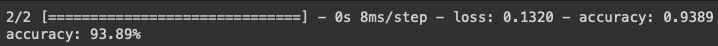
\includegraphics[scale=0.55]{img/evaluateModel.png}
\centering
\caption{Evaluation model results}
\end{figure}
Graph that represent accuracy over the time of epochs. As seen at the begging graph stars in 85\% and then raises to 90\% to 92\%. There is a bit of overfitting in the represented graph. Different methods were tried to reduce that but difference of 1\% to 2\% between training and validation is the best result that came out.
\begin{figure}[H]
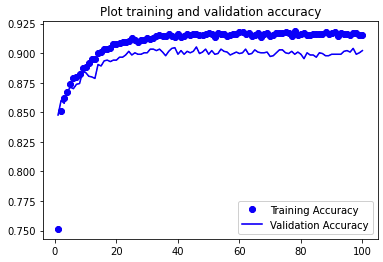
\includegraphics[scale=0.7]{img/trainingAndValidationAccuracy.jpeg}
\centering
\caption{Representation of training and validation accuracy}
\end{figure}
Representation of loss graph is showcasing training and validation difference. As the graph is showcasing, training and validation are on point.
\begin{figure}[H]
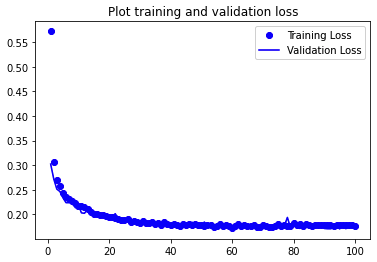
\includegraphics[scale=0.7]{img/trainingAndValidationLoss.jpeg}
\centering
\caption{Representation of training and validation loss}
\end{figure}
With the help of SkLearn library, multi label confusion matrix is calculated and shown. There are 4 things that are represented:
\begin{itemize}
    \item precision
    \item recall
    \item f1-score
    \item support
\end{itemize}
Calculations are done of micro, macro, weighted and samples. With that, we can see different calculations based on different scenarios.
\begin{figure}[H]
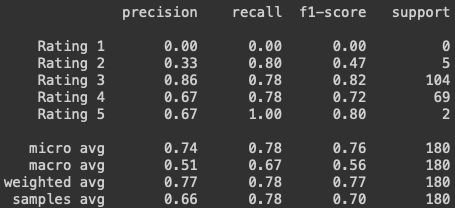
\includegraphics[scale=0.7]{img/clculationConfusionMatrix.jpeg}
\centering
\caption{Representation of calculation confusion matrix}
\end{figure}
Last figure represents multi label confusion matrix. Each label is represented separately. 
\begin{figure}[H]
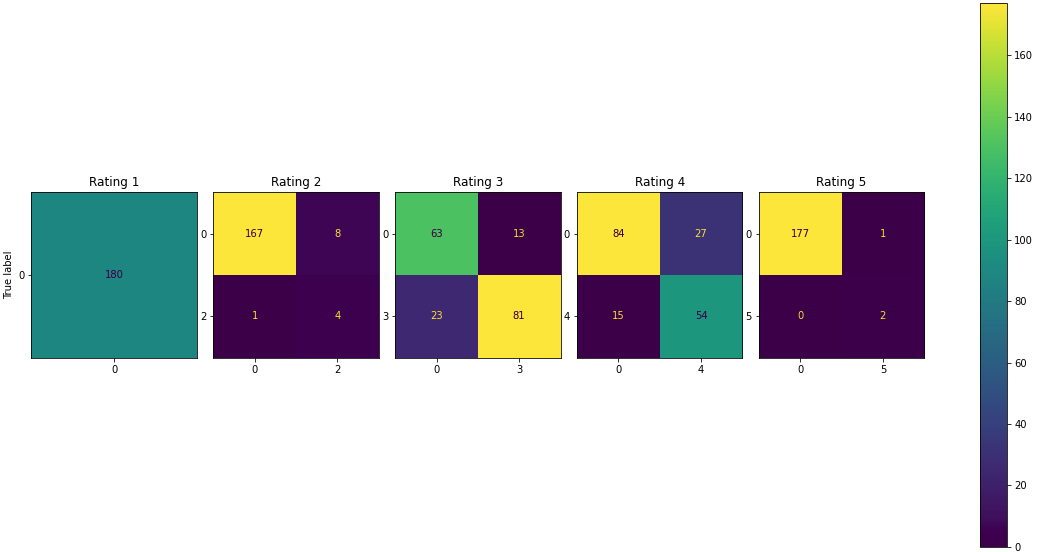
\includegraphics[scale=0.39]{img/visualiseConfusionMatrix.jpeg}
\centering
\caption{Representation of visualise confusion matrix}
\end{figure}